\section{Source, scope, and intended audience}

\subsection{The primary source}

The primary source is Julia Kempe's public lecture \emph{Synthetic Data -- Friend or Foe in the Age of Scaling?}, part of the IHES/CNRS series \emph{Mathematics for and by Large Language Models} \citep{kempevideo2024,ihesmathllm2024}. The lecture develops a scaling-law perspective on synthetic-data training, moving from empirical neural scaling, heavy-tailed data, and the Hutter memory model to recursive model collapse, kernel regression, real/synthetic mixtures, grokking, and verifier-based recovery.

This report does not reproduce the lecture slides. All diagrams are original reconstructions intended to explain the ideas and connect them to the author's companion research programmes. The report also relies on the cited primary papers, especially \citet{dohmatob2024tails}, \citet{dohmatob2024regression}, \citet{feng2025verification}, and \citet{dohmatob2025strong}.

\subsection{What kind of audience was the lecture designed for?}

The event context and mathematical content indicate a research-oriented audience: mathematicians, theoretical computer scientists, machine-learning researchers, and advanced graduate students. The lecture is nevertheless unusually valuable for engineers because its central failure modes can be understood without reproducing every proof.

\begin{figure}[H]
\centering
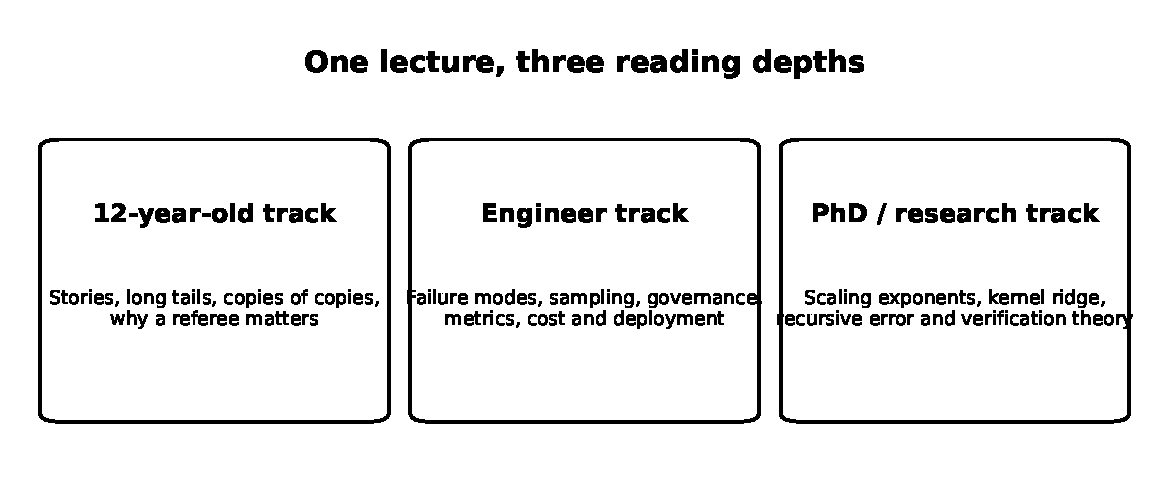
\includegraphics[width=0.95\textwidth]{figures/audience_ladder.pdf}
\caption{Three reading depths used in this document.}
\label{fig:audience}
\end{figure}

The following audience map is therefore appropriate.

\begin{longtable}{p{0.20\textwidth}p{0.35\textwidth}p{0.35\textwidth}}
\toprule
\textbf{Reader} & \textbf{What can be understood directly} & \textbf{What requires additional background} \\
\midrule
Twelve-year-old & Copies of copies lose unusual details; a referee can keep only correct attempts; more examples are not always more knowledge. & Probability laws, asymptotics, ridge regression, autoregressive likelihoods. \\
Engineer & Tail coverage, pseudo-label drift, sampling controls, verification economics, evidence lineage, deployment risks. & Formal scaling exponents, kernel spectra, high-dimensional limits. \\
Graduate / PhD & Derivations, asymptotic regimes, recursive error terms, verifier phase transitions, modified scaling laws. & Full proofs and extensions beyond the paper assumptions. \\
Research programme owner & How to turn these results into hypotheses, metrics, benchmarks, governance and architecture. & Empirical validation on the target system. \\
\bottomrule
\end{longtable}

\subsection{What this document is and is not}

This report is four things at once:

\begin{enumerate}[leftmargin=*]
  \item a pedagogical guide to the lecture;
  \item a technical synthesis of the associated papers;
  \item a critical orientation for \MMALS, \STRATQ, probabilistic MTP, and Test Data Governance;
  \item a reproducible experimental roadmap.
\end{enumerate}

It is not:

\begin{itemize}[leftmargin=*]
  \item a verbatim transcript;
  \item a claim that every practical synthetic-data pipeline collapses;
  \item a proof that MMALS already exhibits or avoids the proposed phenomena;
  \item an official biography or exhaustive map of Julia Kempe's collaborators;
  \item a replacement for reading the original papers.
\end{itemize}

\begin{cautionbox}
Several conclusions in this report are research hypotheses for MMALS and STRAT-Q. They are deliberately marked as orientations rather than validated results. The correct next step is controlled experimentation, not architectural overclaiming.
\end{cautionbox}
